% !TeX program = xelatex
\documentclass[sigconf,nonacm,screen]{acmart}
\usepackage{styles/course-report}
\usepackage{amsmath,booktabs,array,multirow}
\setcitestyle{super,square,comma}
\title[数据挖掘导论课程报告]{数据挖掘导论课程报告}
\begin{document}\maketitle
\section{跨模态正常参考的异常检测方法}
图像异常检测与甲状腺异常判断分别面向空间图像和结构化数值数据。二者输入形式不同，但都可以通过学习正常样本的共同规律，衡量待测样本与正常参考之间的差异。本文以正常参考距离为共同检测核心，并结合各模态的数据特点设计特征转换与阈值确定方法。
\subsection{任务定义与模态差异}
图像输入为RGB像素阵列，缺陷可能只存在于局部区域；同一产品的纹理和拍摄差异也可能产生较大响应。甲状腺输入为六维脱敏数值，异常表现为属性数值或属性关系的偏离，单个样本没有图像那样的空间网格。图像训练集同时包含正常和异常图像，甲状腺训练集仅含正常样本，因此两者可使用的监督信息不同。

两项任务均以异常为正类，目标是输出异常分数与标签。将第$c$种数据的观测记为$x$，其模态适配器记为$\phi_c$，正常参考集合为$\mathcal R_c$，统一检测形式为
\begin{equation} r_c(x)=A_c\!\left(\{d_c(\phi_c(x)_j,\mathcal R_c)\}_j\right),\quad S_c(x)=g_c(r_c(x),x). \end{equation}
其中$A_c$聚合一个样本内的局部分数，$g_c$表示可选的模态适配：甲状腺使用$S_c=r_c$，图像将$r_c$与有监督分支融合。给定该类别的阈值$\tau_c$，正常参考模型以$S_c(x)>\tau_c$判定异常，图像监督融合则使用$S_c(x)\geq\tau_c$。分数与阈值分别在各数据集上确定，不直接比较不同模态的原始距离。
\begin{figure*}[t]\centering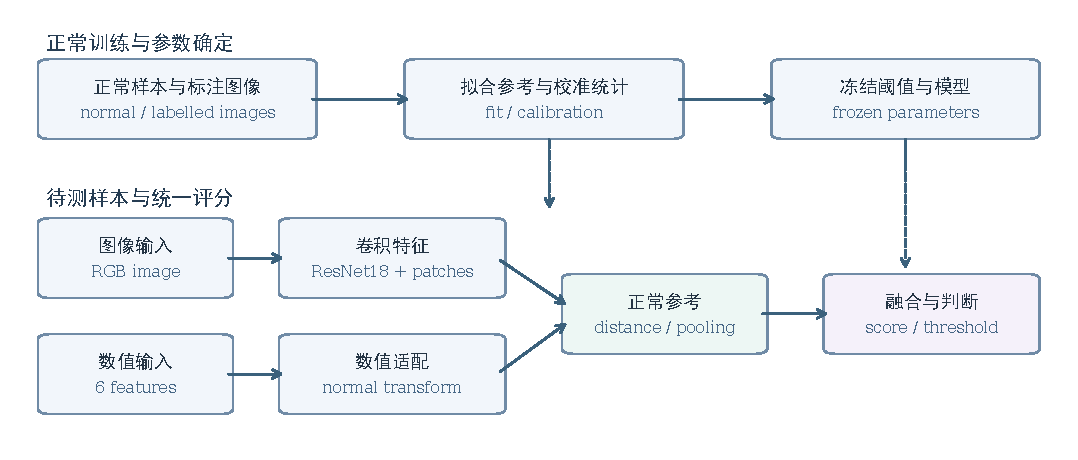
\includegraphics[width=\textwidth]{figures/framework.pdf}\caption{跨模态异常检测框架。两种输入通过各自适配器进入正常参考评分，图像还可利用训练异常标签进行分数修正。}\label{fig:framework}\end{figure*}

\subsection{统一框架与设计思想}
图\ref{fig:framework}展示统一流程：先由不同的特征适配器把原始输入转成数值描述子，再根据正常数据建立参考、计算距离并聚合为样本分数，最后根据训练数据确定判定阈值。统一的是正常参考评分与样本级判定流程；特征表示、参考构造和可用标签仍须适应各模态。

近邻方法以样本距离描述局部相似性\cite{cover1967}；本文借用这一思想度量偏离，而非直接进行近邻分类。对描述子$\mathbf z_j$，一般正常参考分支计算到$k$个最近正常参考的平均距离：
\begin{equation} d_j=\frac{1}{k\sqrt D}\sum_{r\in N_k(\mathbf z_j)}\lVert\mathbf z_j-\mathbf r\rVert_2.\end{equation}
图像由多个局部描述子组成，取分数最高的$\lceil 0.02m\rceil$个距离求均值；当数值样本只产生一个描述子时，聚合自然退化为单个距离。参考库、变换参数及聚合规则均在训练阶段确定。距离除以$\sqrt D$用于缓和维数变化对距离尺度的影响。图像的高分局部区域可能对应缺陷，故使用上尾均值；这一选择也可能对背景变化和噪声敏感。各类别分别构建参考库与阈值，不要求图像和表格的原始分数具有相同量纲。

\subsection{图像与数值特征处理}
图像数据缩放到$256\times256$，采用冻结的预训练ResNet18\cite{he2016}提取全局特征和局部特征。局部特征形成$16\times16$、每个64维的描述子网格，正常参考库最多保留8192个描述子；正常参考分支使用$k=5$。考虑训练集中存在异常标签，最终图像方法进一步使用支持向量机学习全局正常与异常差异，将其分数与正常参考分数校准后融合，固定候选范围内的权重及阈值由训练内折外结果确定。拉链分支的候选范围曾依据课程测试结果比较确定。

两个图像分支的分数尺度不同。记训练集正常图像折外分数的中位数和四分位距为$m_b$和$I_b$，分支$b$的校准分数为$\widetilde s_b=(s_b-m_b)/I_b$。设支持向量机权重为$w$，则最终分数为
\begin{equation}S_{\mathrm{img}}=w\widetilde s_{\mathrm{SVM}}+(1-w)\widetilde s_{\mathrm{local}}.\end{equation}
两类分别进行分层五折训练内评分；冻结配置后使用全部训练图像重拟合。榛子最终$w=0.5$，拉链最终$w=0.95$。训练内折外阈值是经验工作点，不将其解释为独立测试保证。每折只用其余四折拟合分支，再对留出折打分；合并留出折的分数后比较候选权重并选择F1工作点。每个用于选阈值的训练样本分数来自未用该样本拟合的模型，但候选范围和方法开发过程仍可能引入选择偏差。最终模型用全部训练数据重拟合，测试标签不用于拟合参数。

甲状腺数据先对正常训练记录去重，再将正常样本拆成拟合与校准两部分。最终适配器选择第2、6列，使用正常拟合数据学习Yeo--Johnson变换\cite{yeo2000}及稳健缩放，构造方向联合偏离描述子
\begin{equation} u(x)=\max(z_2,0)\max(-z_6,0). \end{equation}
正常参考取该描述子的正常中位数，实际拟合值为0，采用一维曼哈顿距离评分。357条正常校准记录用于确定上尾阈值，最终$\alpha=0.005$，分数严格大于阈值判为异常。特征选择、方向和阈值比例曾依据课程测试结果比较，故属于探索性设计，并非独立盲测结论。该描述子只有在第2列向正方向且第6列向负方向同时偏离时才为正；若仅一个方向发生变化，乘积可能为零，因此可能漏掉其他异常模式。稳健缩放以正常拟合数据的中位数和第10至90百分位范围为依据；校准数据不参与变换参数拟合，用于确定正常分数上尾的阈值。

\subsection{实验}
\subsubsection{数据预处理与划分}
榛子和拉链训练集各含200张正常及50张异常图，测试集分别有55张和47张图像。甲状腺训练集1839条均为正常，去重后1782条，其中1425条用于正常拟合、357条用于校准；测试集含1839条正常、94条异常，共1933条。训练与测试之间有56条相同正常记录，因此额外报告移除这些测试记录后的结果。

\begin{table}[t]\caption{跨模态数据划分与类别构成（条）}\label{tab:data}\centering\setlength{\tabcolsep}{3pt}
\begin{tabular}{lrrrr}\toprule
&\multicolumn{2}{c}{训练集}&\multicolumn{2}{c}{测试集}\\
\cmidrule(lr){2-3}\cmidrule(lr){4-5}
数据&正常&异常&正常&异常\\\midrule
榛子&200&50&40&15\\
拉链&200&50&32&15\\
甲状腺&1839&0&1839&94\\\bottomrule
\end{tabular}\end{table}

\subsubsection{实验配置与拟合流程}
本次在Windows 11、Python 3.12.14的CPU环境下完整重新运行，使用4个计算线程和批大小8。图像输入先经共享编码器提取特征，再分别拟合正常参考和监督分支；表格输入仅以正常训练样本拟合变换与正常参考。分数和预测在关联测试标签前保存，随后计算评价指标。具体依赖、冻结参数及逐样本结果见随附实验记录。实验随机种子为42。图像的正常参考局部分数与全局监督分数分别计算，用训练内正常样本的折外分数做稳健尺度校准后加权融合；表格数据先去重再拆分拟合和校准集，避免重复记录同时进入两部分。各数据集分别保存分数、阈值和预测结果，便于复查指标。

\subsubsection{评价指标}

评价以异常为正类，计算精确率、召回率、F1、AUROC及平均精确率AP。记真正例、假正例和假负例分别为TP、FP、FN，则
\begin{equation} P=\frac{TP}{TP+FP},\quad R=\frac{TP}{TP+FN},\quad F1=\frac{2PR}{P+R}. \end{equation}
ROC与PR曲线从不同角度描述排序表现\cite{davis2006}；AUROC和AP评价连续分数的排序能力；F1等指标反映固定阈值下的实际判定。基线使用全局表示上的PCA近邻与残差评分，正常参考方法使用相应模态的正常参考分支，适配方法为本文最终图像融合与甲状腺方向联合偏离方法。
\begin{table*}[t]\caption{不同方法在课程原始测试集上的效果}\label{tab:results}\centering\setlength{\tabcolsep}{4pt}
\begin{tabular}{llrrrrrr}
\toprule
数据&方法&TN/FP/FN/TP&Precision&Recall&F1&AUROC&AP\\\midrule
榛子 & 基线 & 39/1/1/14 & 0.9333 & 0.9333 & 0.9333 & 0.9967 & 0.9922 \\
榛子 & 正常参考 & 40/0/2/13 & 1.0000 & 0.8667 & 0.9286 & 1.0000 & 1.0000 \\
榛子 & 适配方法 & 40/0/0/15 & 1.0000 & 1.0000 & 1.0000 & 1.0000 & 1.0000 \\
拉链 & 基线 & 29/3/6/9 & 0.7500 & 0.6000 & 0.6667 & 0.9042 & 0.8107 \\
拉链 & 正常参考 & 29/3/1/14 & 0.8235 & 0.9333 & 0.8750 & 0.9563 & 0.8991 \\
拉链 & 适配方法 & 32/0/0/15 & 1.0000 & 1.0000 & 1.0000 & 1.0000 & 1.0000 \\
甲状腺 & 基线 & 1746/93/7/87 & 0.4833 & 0.9255 & 0.6350 & 0.9772 & 0.7972 \\
甲状腺 & 正常参考 & 1819/20/26/68 & 0.7727 & 0.7234 & 0.7473 & 0.9766 & 0.7958 \\
甲状腺 & 适配方法 & 1833/6/1/93 & 0.9394 & 0.9894 & 0.9637 & 0.9958 & 0.9615 \\
\bottomrule
\end{tabular}
\end{table*}
\begin{figure*}[t]\centering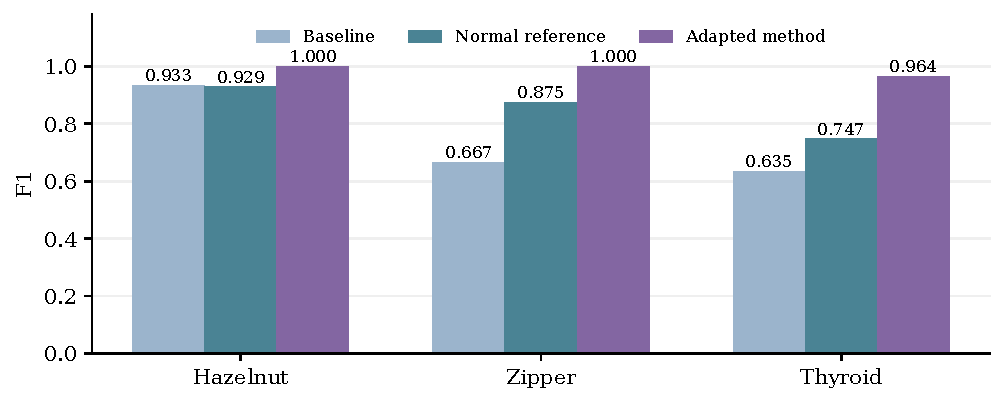
\includegraphics[width=\textwidth]{figures/comparison.pdf}\caption{三种方法的F1对比。Baseline、Normal reference和Adapted method分别表示基线、正常参考及适配方法。}\label{fig:comparison}\end{figure*}
\begin{figure*}[t]\centering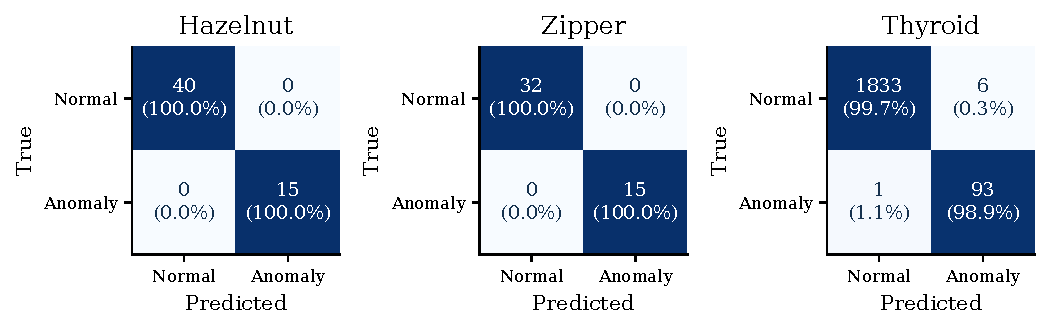
\includegraphics[width=\textwidth]{figures/confusion.pdf}\caption{最终方法的混淆矩阵。Normal表示正常，Anomaly表示异常；行是真实类别，列是预测类别，括号内为行比例。}\label{fig:confusion}\end{figure*}
\begin{figure*}[t]\centering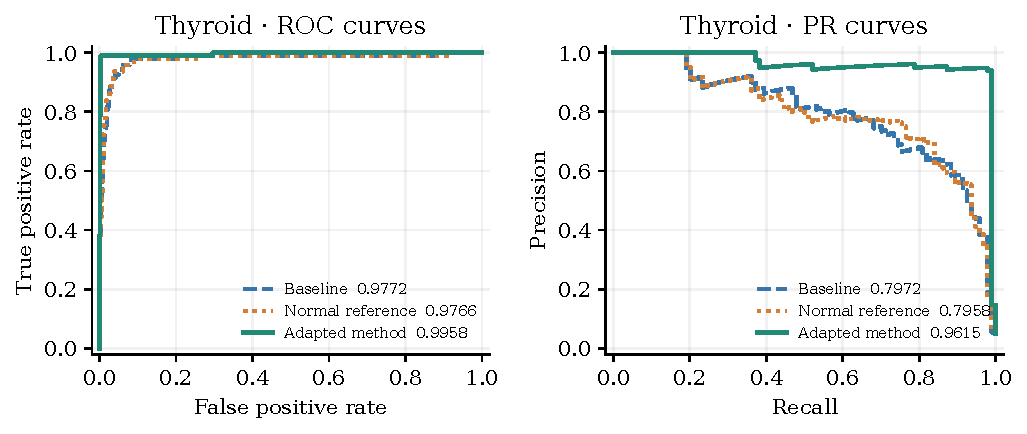
\includegraphics[width=\textwidth]{figures/thyroid-roc-pr.pdf}\caption{甲状腺测试集中基线、正常参考和适配方法的ROC与PR曲线。图例数值分别为AUROC与AP。}\label{fig:curves}\end{figure*}
\begin{figure*}[t]\centering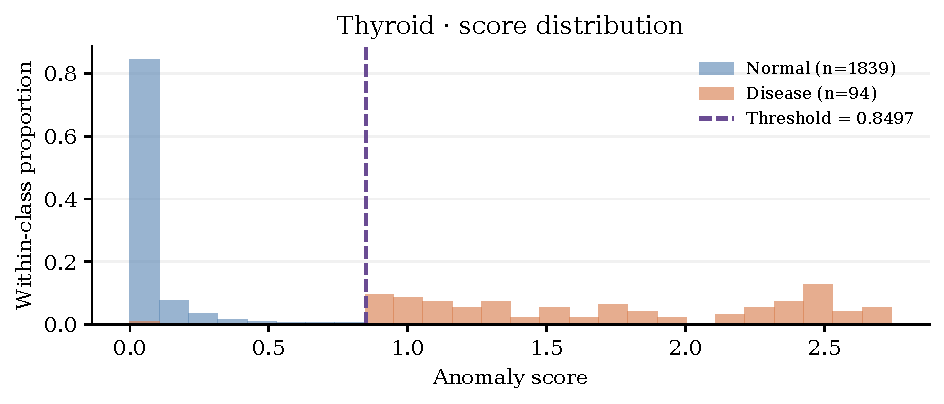
\includegraphics[width=0.85\textwidth]{figures/thyroid-score-distribution.pdf}\caption{甲状腺测试集的异常分数分布。Normal为正常，Disease为患病；纵轴为类内比例，虚线为校准阈值。}\label{fig:distribution}\end{figure*}

\subsubsection{实验结果与分析}
表\ref{tab:results}和图\ref{fig:comparison}给出三种方法的结果。图像最终方法对榛子55张、拉链47张测试图均判断正确，合计102/102；甲状腺原始测试集为1833个TN、6个FP、1个FN和93个TP，F1为0.9637，AUROC为0.9958。图\ref{fig:confusion}展示各数据集的判定结果。图像结果使用异常训练标签，不能将其直接归因于纯无监督方法。

甲状腺测试集中有56条正常记录与训练集相同。移除后剩余1877条，最终方法的混淆计数为1777个TN、6个FP、1个FN和93个TP，F1仍为0.9637，AUROC为0.9956。该对照说明这些重复记录对本次精确率、召回率和F1没有改变，但不能消除开发过程中使用测试结果进行方法比较造成的偏差。

从适配差异看，正常参考方法为图像提供局部偏离线索；融合分支利用已有异常标签改进图像级判断。甲状腺的方向联合描述子强调两个选定变量同时沿指定方向偏离正常参考。两者说明统一检测核心能够承接不同类型的数值表示，也说明特征提取与监督方式不宜强行完全一致。拉链正常参考的F1为0.8750，融合后为1.0000；甲状腺正常参考的F1为0.7473，方向联合描述子达到0.9637。这些差异同时包含特征设计、阈值和监督条件变化，不能单独视为某一组件的因果贡献。榛子正常参考的AUROC已为1.0000，但固定阈值下仍漏检2例，体现排序质量与固定阈值分类质量并不等价。

图\ref{fig:curves}给出甲状腺数据的ROC与PR曲线。适配方法的AUROC和AP分别为0.9958和0.9615，高于两种对照；曲线描述不同阈值下的排序效果，固定阈值的误报与漏检仍需结合混淆矩阵判断。图\ref{fig:distribution}展示两类记录的分数分布，大多数正常记录位于阈值左侧；6条正常记录超过阈值，1条患病记录未超过阈值。阈值敏感性记录显示，$\alpha$从0.005改为0.01、0.02和0.05时，误报分别由6增至22、32和76，漏报均为1，F1分别降至0.8900、0.8493和0.7072；排序分数不变，AUROC与AP也不变。这说明工作点会改变误报与精确率，不能仅凭排序指标选择判定规则。

本次重新运行后，使用保存的模型和独立核验程序对602张原始图像重新提取全局与局部特征，最大差均为0；对14041行预测、24行指标和1588条校准分数进行了复核。新旧逐样本预测文件的SHA256一致。实验具有数据量有限、测试集曾参与开发选择等限制，不能据此保证对新产品、未知缺陷或外部医疗数据的表现。图像测试各仅有15个异常样本，一例错误即可明显改变召回率；甲状腺类别不均衡，准确率可能被多数类主导，因此同时报告精确率、召回率及AP。后续应先固定特征、候选范围和阈值策略，再在独立数据上评估，并分别检验不同缺陷与采集条件。
\FloatBarrier
\subsection{小结}
图像与表格异常检测可以统一为“模态适配、正常参考评分、样本级聚合和阈值判定”的流程。保留模态特有的特征表示和监督条件，可以兼顾跨模态框架的复用性与任务差异。后续应在未参与方法选择的独立数据上评估稳定性，并检验不同采集条件和异常类型下的泛化能力。
\newpage
\bibliographystyle{ACM-Reference-Format}
\bibliography{bib/course-report-references}
\end{document}
